% Options for packages loaded elsewhere
\PassOptionsToPackage{unicode}{hyperref}
\PassOptionsToPackage{hyphens}{url}
\documentclass[
  10pt,
  a4paper]{article}
\usepackage{xcolor}
\usepackage[margin=2.5cm]{geometry}
\usepackage{amsmath,amssymb}
\setcounter{secnumdepth}{5}
\usepackage{iftex}
\ifPDFTeX
  \usepackage[T1]{fontenc}
  \usepackage[utf8]{inputenc}
  \usepackage{textcomp} % provide euro and other symbols
\else % if luatex or xetex
  \usepackage{unicode-math} % this also loads fontspec
  \defaultfontfeatures{Scale=MatchLowercase}
  \defaultfontfeatures[\rmfamily]{Ligatures=TeX,Scale=1}
\fi
\usepackage{lmodern}
\ifPDFTeX\else
  % xetex/luatex font selection
\fi
% Use upquote if available, for straight quotes in verbatim environments
\IfFileExists{upquote.sty}{\usepackage{upquote}}{}
\IfFileExists{microtype.sty}{% use microtype if available
  \usepackage[]{microtype}
  \UseMicrotypeSet[protrusion]{basicmath} % disable protrusion for tt fonts
}{}
\makeatletter
\@ifundefined{KOMAClassName}{% if non-KOMA class
  \IfFileExists{parskip.sty}{%
    \usepackage{parskip}
  }{% else
    \setlength{\parindent}{0pt}
    \setlength{\parskip}{6pt plus 2pt minus 1pt}}
}{% if KOMA class
  \KOMAoptions{parskip=half}}
\makeatother
\usepackage{longtable,booktabs,array}
\usepackage{calc} % for calculating minipage widths
% Correct order of tables after \paragraph or \subparagraph
\usepackage{etoolbox}
\makeatletter
\patchcmd\longtable{\par}{\if@noskipsec\mbox{}\fi\par}{}{}
\makeatother
% Allow footnotes in longtable head/foot
\IfFileExists{footnotehyper.sty}{\usepackage{footnotehyper}}{\usepackage{footnote}}
\makesavenoteenv{longtable}
\usepackage{graphicx}
\makeatletter
\newsavebox\pandoc@box
\newcommand*\pandocbounded[1]{% scales image to fit in text height/width
  \sbox\pandoc@box{#1}%
  \Gscale@div\@tempa{\textheight}{\dimexpr\ht\pandoc@box+\dp\pandoc@box\relax}%
  \Gscale@div\@tempb{\linewidth}{\wd\pandoc@box}%
  \ifdim\@tempb\p@<\@tempa\p@\let\@tempa\@tempb\fi% select the smaller of both
  \ifdim\@tempa\p@<\p@\scalebox{\@tempa}{\usebox\pandoc@box}%
  \else\usebox{\pandoc@box}%
  \fi%
}
% Set default figure placement to htbp
\def\fps@figure{htbp}
\makeatother
\setlength{\emergencystretch}{3em} % prevent overfull lines
\providecommand{\tightlist}{%
  \setlength{\itemsep}{0pt}\setlength{\parskip}{0pt}}
\usepackage{bookmark}
\IfFileExists{xurl.sty}{\usepackage{xurl}}{} % add URL line breaks if available
\urlstyle{same}
\hypersetup{
  pdftitle={Test 005: Put a labeled figure/table inside a theorem/proof etc.},
  pdfauthor={Emma Cliffe, Skills Centre: MASH, University of Bath},
  hidelinks,
  pdfcreator={LaTeX via pandoc}}

\title{Test 005: Put a labeled figure/table inside a theorem/proof etc.}
\author{Emma Cliffe, Skills Centre: MASH, University of Bath}
\date{August 2020}

\usepackage{amsthm}
\theoremstyle{plain}
\newtheorem*{theorem*}{Theorem}\newtheorem{theorem}{Theorem}[section]
\newtheorem*{Thought*}{Thought}\newtheorem{Thought}{Thought}[section]
\theoremstyle{definition}
\newtheorem*{proposition*}{Proposition}\newtheorem{proposition}[theorem]{Proposition}
\newtheorem*{Nugget*}{Nugget}\newtheorem{Nugget}[Thought]{Nugget}
\theoremstyle{plain}
\newtheorem*{lemma*}{Lemma}\newtheorem{lemma}{Lemma}[section]
\theoremstyle{plain}
\newtheorem*{corollary*}{Corollary}\newtheorem{corollary}{Corollary}[section]
\theoremstyle{plain}
\newtheorem*{conjecture*}{Conjecture}\newtheorem{conjecture}{Conjecture}[section]
\theoremstyle{definition}
\newtheorem*{definition*}{Definition}\newtheorem{definition}{Definition}[section]
\theoremstyle{definition}
\newtheorem*{example*}{Example}\newtheorem{example}{Example}[section]
\theoremstyle{definition}
\newtheorem*{exercise*}{Exercise}\newtheorem{exercise}{Exercise}[section]
\newtheorem*{Solution*}{Solution}\newtheorem{Solution}{Solution}[section]
\theoremstyle{remark}
\newtheorem*{remark*}{Remark}
\newtheorem*{solution*}{Solution}
\theoremstyle{plain}
\newtheorem*{Defns*}{Defns}
\newtheorem*{Proof*}{Proof}
\newtheorem*{Exercises*}{Exercises}
\newtheorem*{Example*}{Example}
\let\BeginKnitrBlock\begin \let\EndKnitrBlock\end
\begin{document}
\maketitle

{
\setcounter{tocdepth}{2}
\tableofcontents
}
\section{Here is a figure}\label{here-is-a-figure}

\begin{figure}
\centering
\pandocbounded{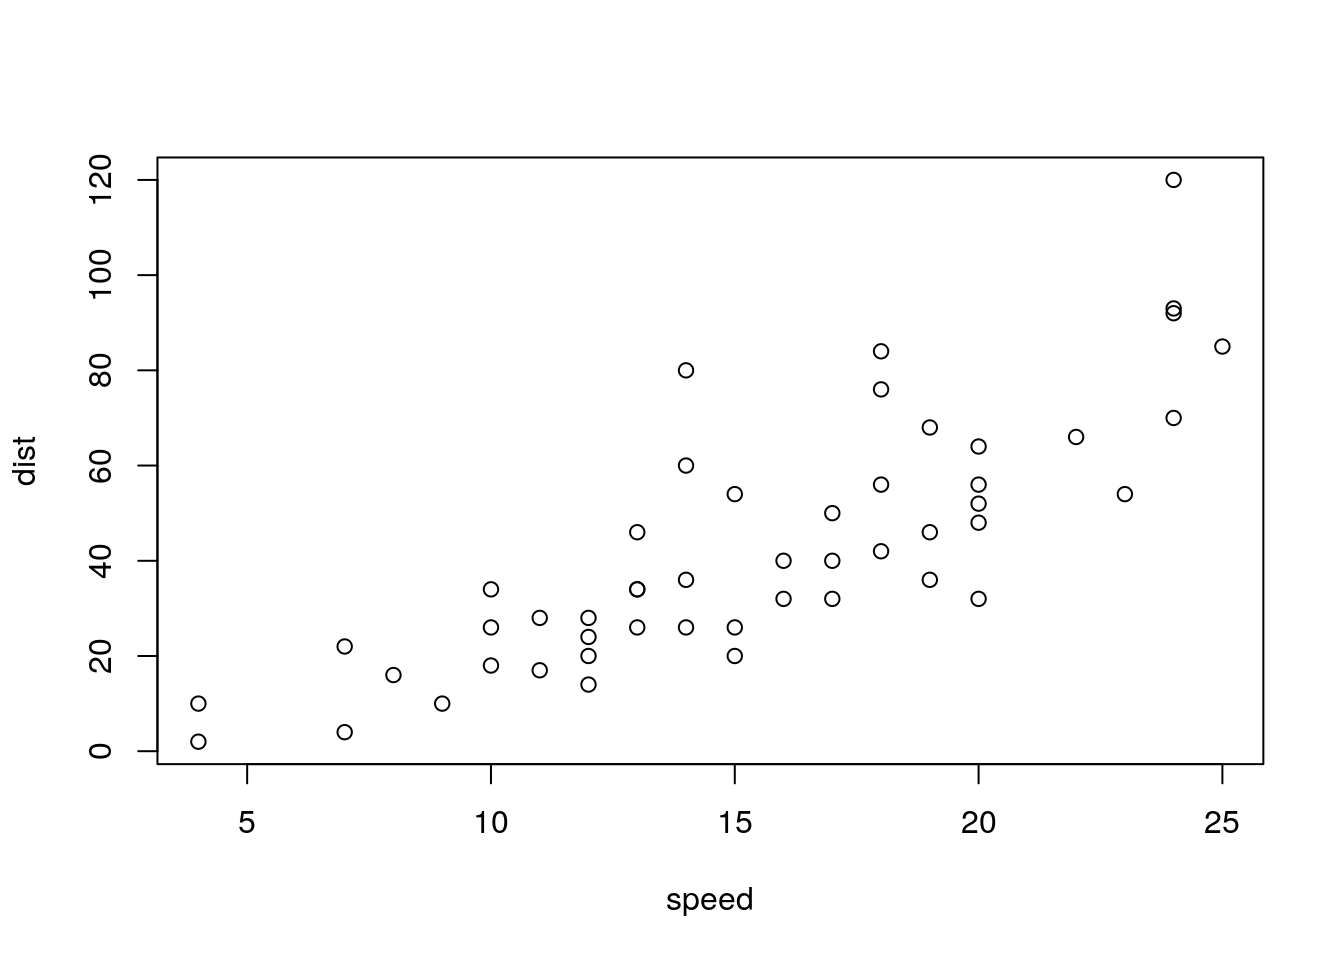
\includegraphics[keepaspectratio,alt={Something else to do with cars}]{Notes_files/figure-html/cars-plot-1.png}}
\caption{\label{fig:cars1}Something else to do with cars}
\end{figure}

\section{Here is the putting of a figure inside another built in environment}\label{here-is-the-putting-of-a-figure-inside-another-built-in-environment}

\BeginKnitrBlock{example}
{\label{exm:unnamed-chunk-1} }Here is an example.

\begin{figure}
\centering
\pandocbounded{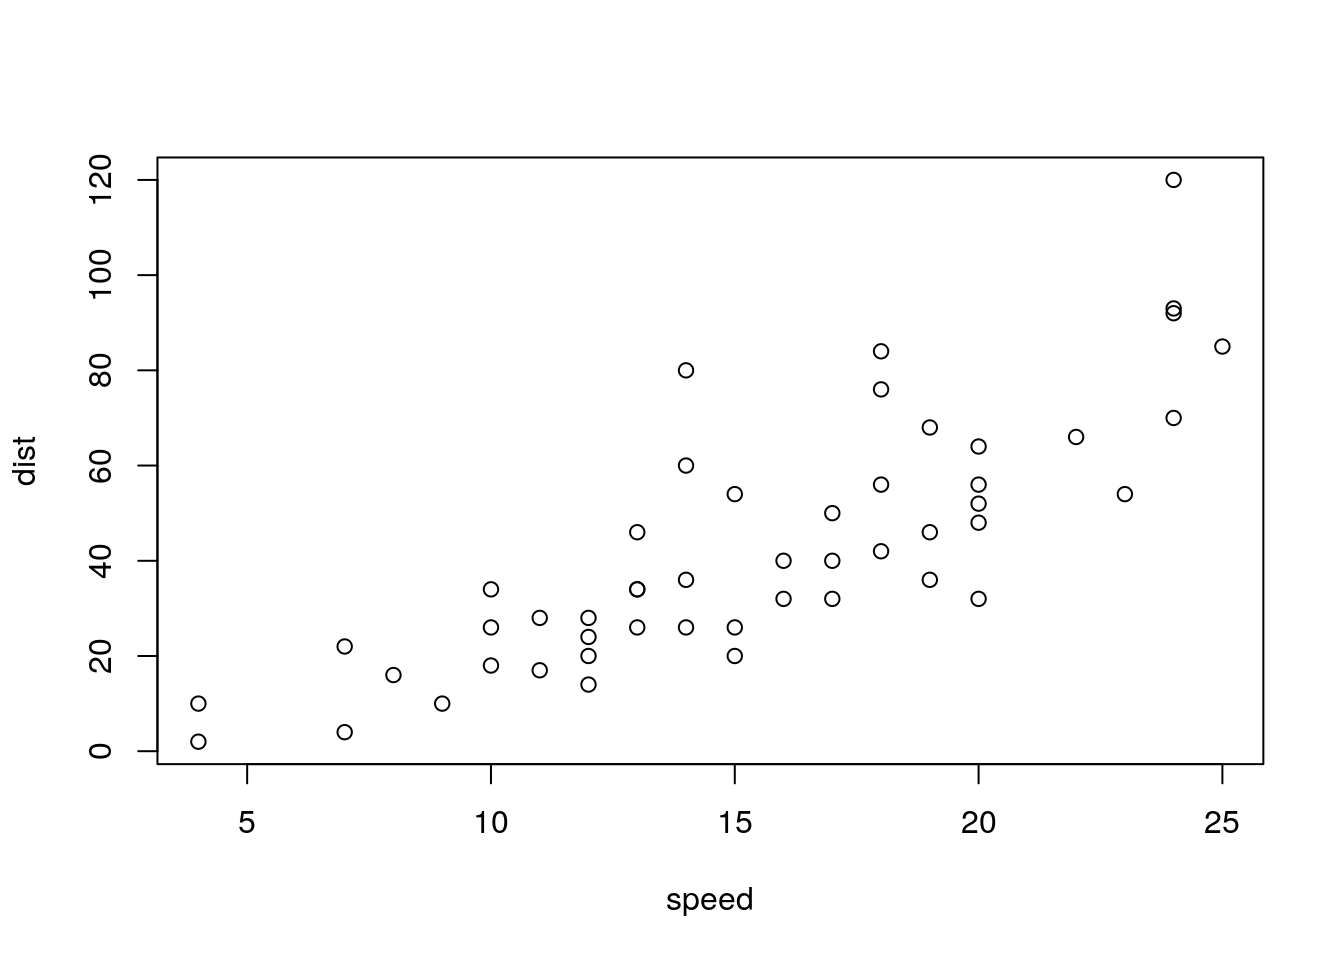
\includegraphics[keepaspectratio,alt={Something to do with cars}]{Notes_files/figure-html/cars-plot-1.png}}
\caption{\label{fig:cars2}Something to do with cars}
\end{figure}

This is a test. So, you need an empty line before and after the above for it to be a float. At the end of an environment this means that you need TWO empty lines. This is Pandoc.
\EndKnitrBlock{example}

\section{Here is the putting of a figure inside a newtheorem}\label{here-is-the-putting-of-a-figure-inside-a-newtheorem}

\BeginKnitrBlock{Example*}
{}An example

\begin{figure}
\centering
\pandocbounded{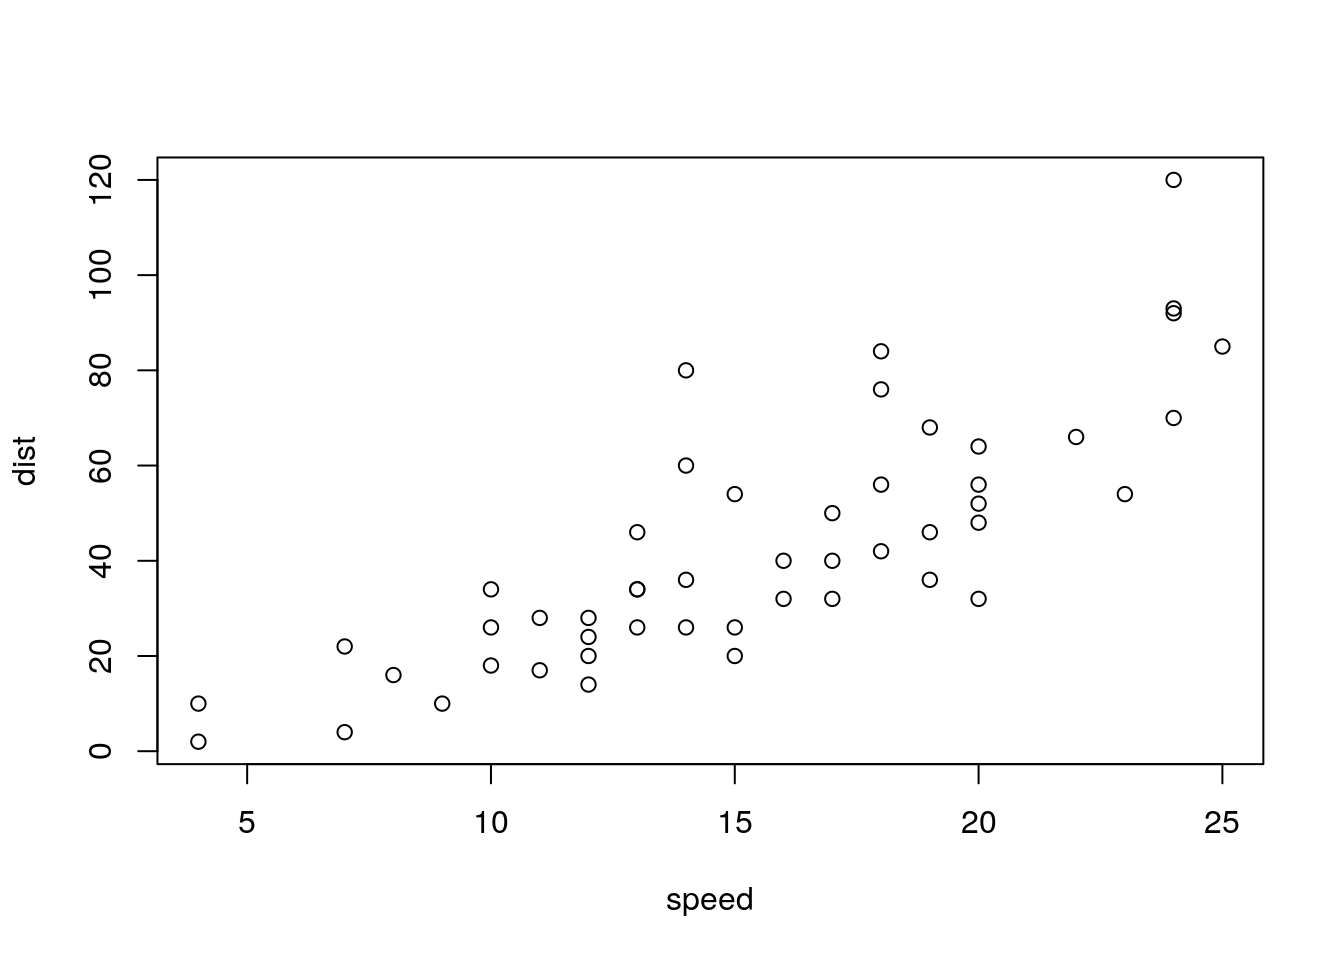
\includegraphics[keepaspectratio,alt={Something to do with cars}]{Notes_files/figure-html/cars-plot-1.png}}
\caption{\label{fig:cars3}Something to do with cars}
\end{figure}
\EndKnitrBlock{Example*}

\section{Here is when we set width - and everything is different now}\label{here-is-when-we-set-width---and-everything-is-different-now}

\begin{figure}
\centering
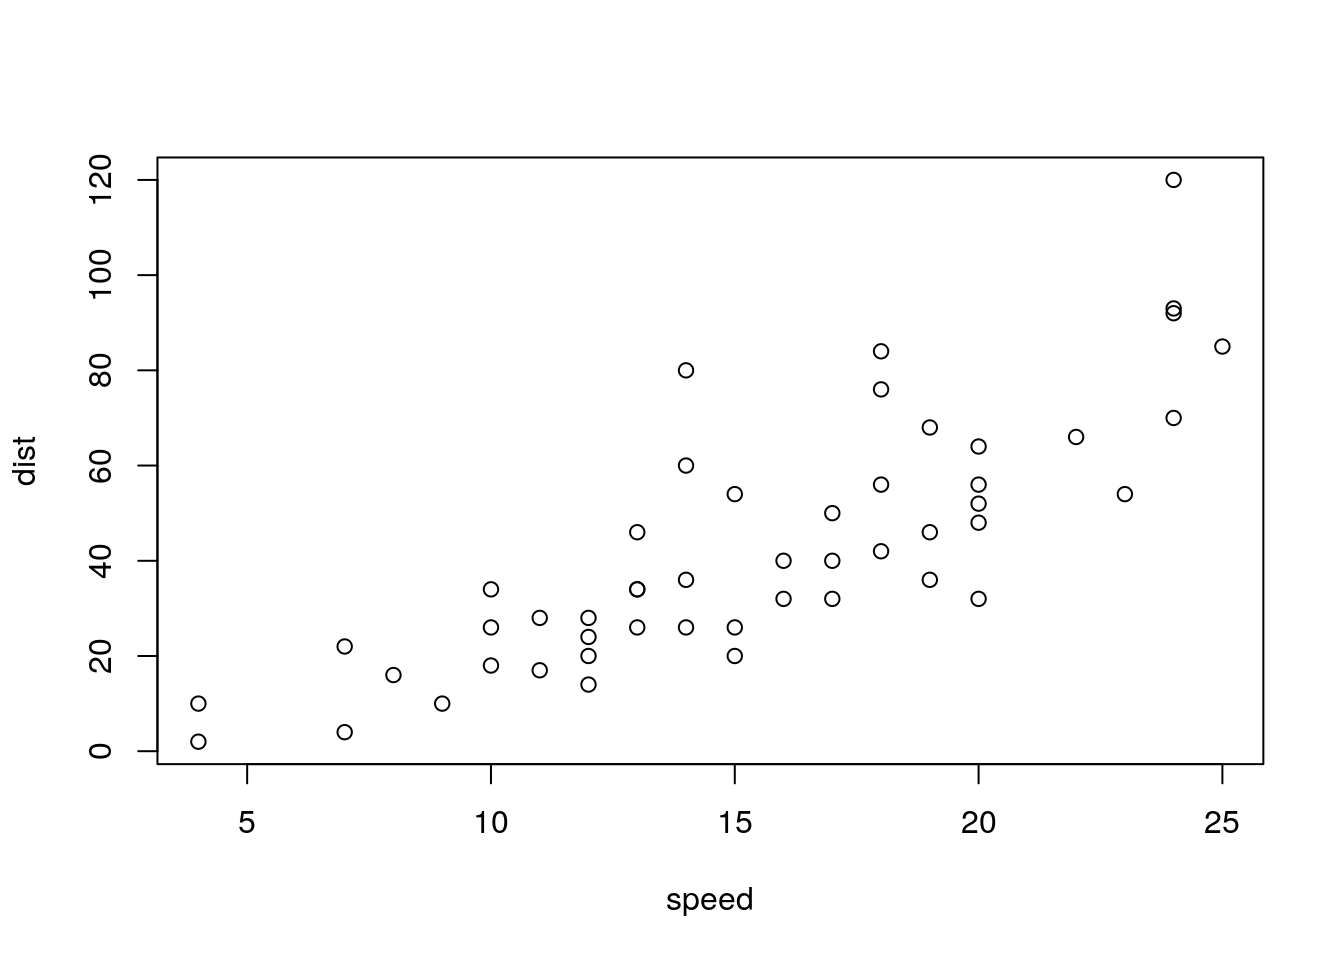
\includegraphics[width=0.6\linewidth,height=\textheight,keepaspectratio,alt={Something else to do with cars}]{Notes_files/figure-html/cars-plot-1.png}
\caption{\label{fig:cars4}Something else to do with cars}
\end{figure}

\end{document}
